\chapter{Applications et étalonnage}
\section{Voltmètre}
Affiche la tension de la batterie en fonctionnement. evo\_v\_l présente une valeur numérique avec une icône de batterie ; iv\_evo\_v\_t utilise un affichage à segments semblable à IV-Nano.

\begin{figure}[H]
\centering
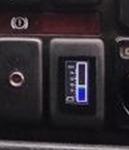
\includegraphics[width=.85\textwidth,height=.60\textheight,keepaspectratio]{figures/ivevo/image16.png}
\caption{Voltmètre}
\end{figure}

\begin{figure}[H]
\centering
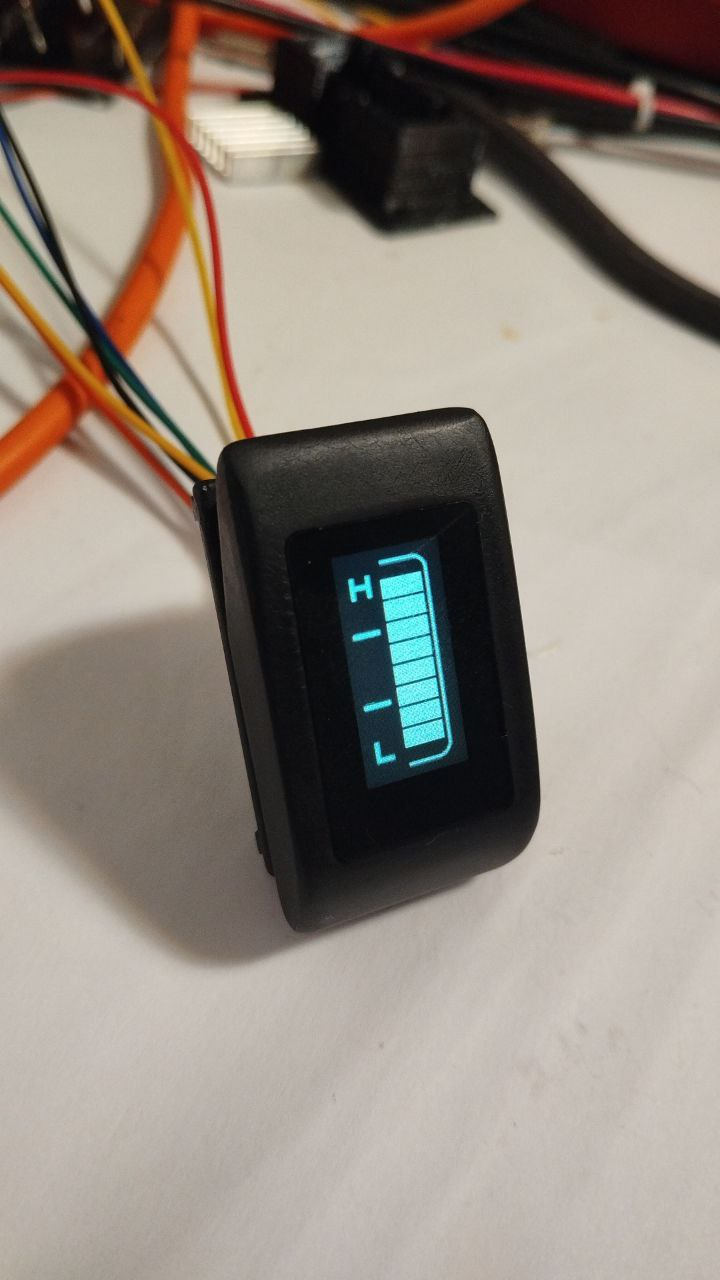
\includegraphics[width=.85\textwidth,height=.60\textheight,keepaspectratio]{figures/ivevo/image15.png}
\caption{Voltmètre}
\end{figure}

\begin{figure}[H]
\centering
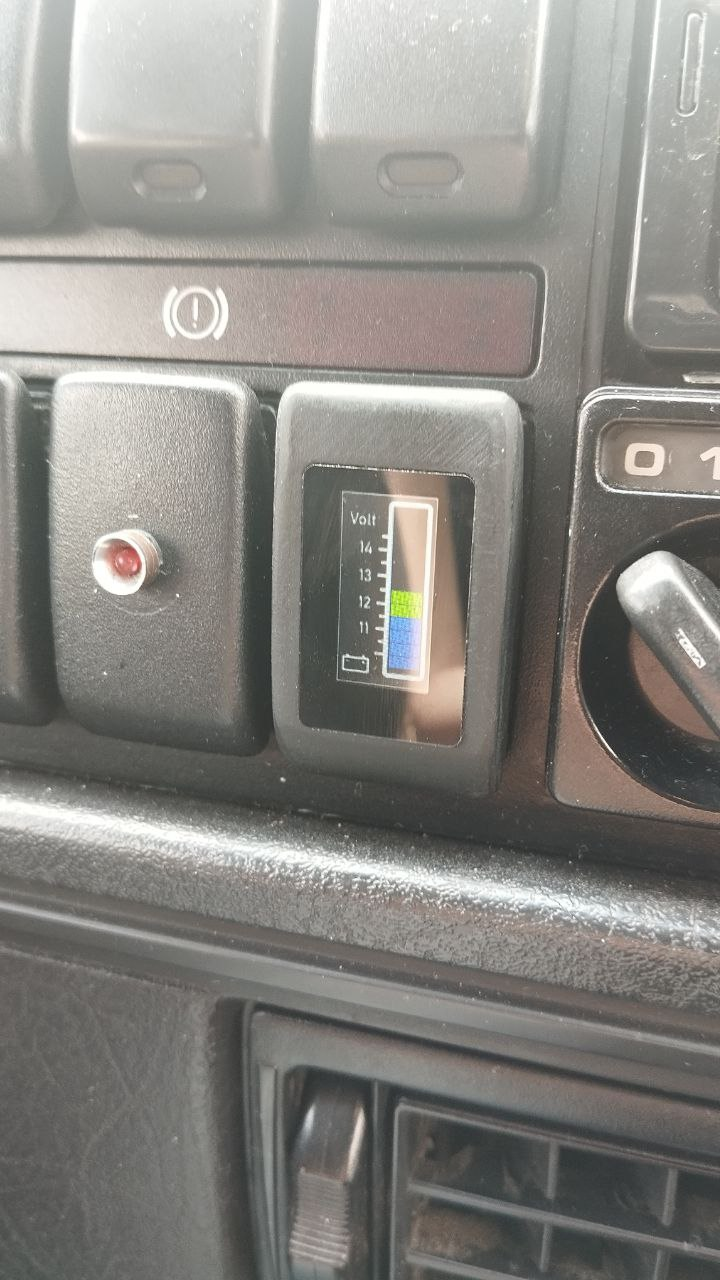
\includegraphics[width=.85\textwidth,height=.60\textheight,keepaspectratio]{figures/ivevo/image2.png}
\caption{Voltmètre}
\end{figure}
\section{Pression d'huile (Barometer)}
Un capteur est obligatoire ; le modèle prévu est VAG 03C906051A. Malgré la sortie +5 V interne, la source recommande un convertisseur DC/DC externe pour le capteur. Suivre le schéma de pression d'huile et utiliser un étalonnage adapté au capteur.

\begin{figure}[H]
\centering
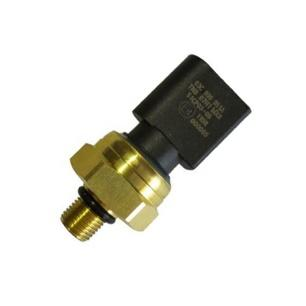
\includegraphics[width=.85\textwidth,height=.60\textheight,keepaspectratio]{figures/ivevo/image21.jpg}
\caption{Pression d'huile (Barometer)}
\end{figure}
\section{Température (Thermo)}
Choisir un capteur NTC ou un DS18B20 numérique et le script correspondant. Les sondes DS18B20 câblées sont acceptées. Pour le NTC, Ossca 01176 ou un capteur Golf 2 compatible est recommandé. Sur le capteur Ossca, relier les broches du capteur 1 et 2 ; la résistance NTC est raccordée à la broche du capteur 3. Ce sont les numéros du capteur, pas les broches d'alimentation de l'indicateur.

\begin{figure}[H]
\centering
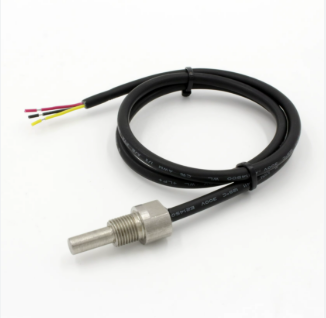
\includegraphics[width=.85\textwidth,height=.60\textheight,keepaspectratio]{figures/ivevo/image14.png}
\caption{Température (Thermo)}
\end{figure}

\begin{figure}[H]
\centering
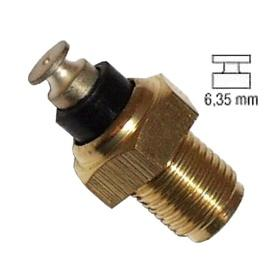
\includegraphics[width=.85\textwidth,height=.60\textheight,keepaspectratio]{figures/ivevo/image19.jpg}
\caption{Température (Thermo)}
\end{figure}
\section{Indicateur de rapport}
Affiche R et les rapports 1–5. Il calcule le rapport à partir de la vitesse et du régime reçus de Digifiz Next par Bluetooth LE. La marche arrière nécessite un signal positif sur une entrée conformément au schéma. Digifiz Next doit disposer du micrologiciel 1.0.14 ou ultérieur.

Pour cette application, raccorder la broche 1 (K30/KL30) au +12 V KL15 après contact et la broche 7 à la masse. Au démarrage, un tiret signifie qu'aucun rapport n'est sélectionné ; l'appareil recherche Digifiz Next. En mode QR, choisir l'application iv\_gear et le capteur volts1, enregistrer et remettre le contact.

Dans le panneau web Digifiz Next, étalonner la vitesse avec le GPS, le régime et la table des rapports selon le véhicule. La source suggère 80–100 km/h comme référence : uniquement dans des conditions légales et sûres, avec un passager notant les valeurs. Les valeurs de régime 1500, 3000 et 400 n'ont ni unité ni correspondance moteur clairement définies. Consulter les instructions du combiné pour le moteur concerné sans deviner les réglages.

\begin{figure}[H]
\centering
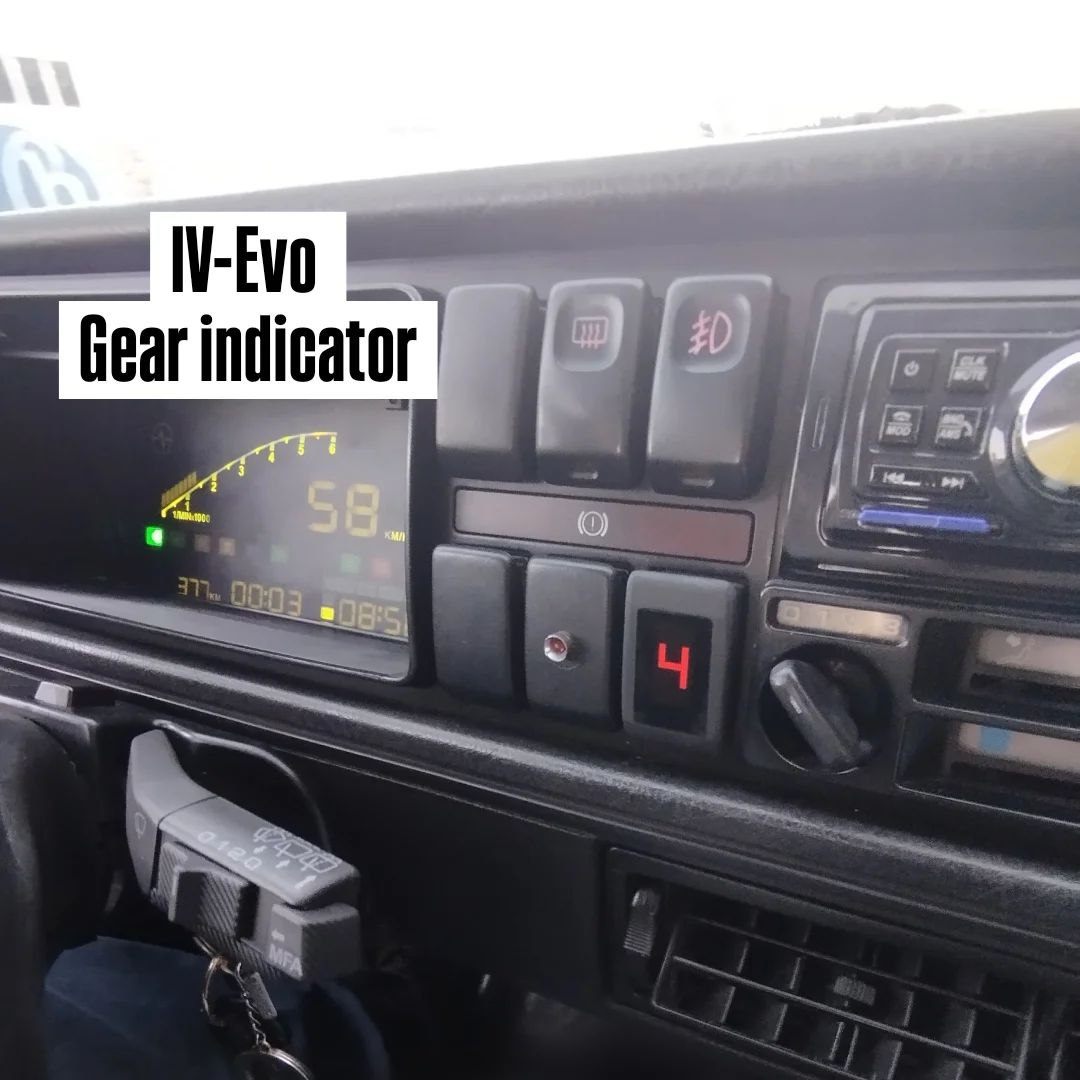
\includegraphics[width=.85\textwidth,height=.60\textheight,keepaspectratio]{figures/ivevo/image18.png}
\caption{Indicateur de rapport}
\end{figure}

\begin{figure}[H]
\centering
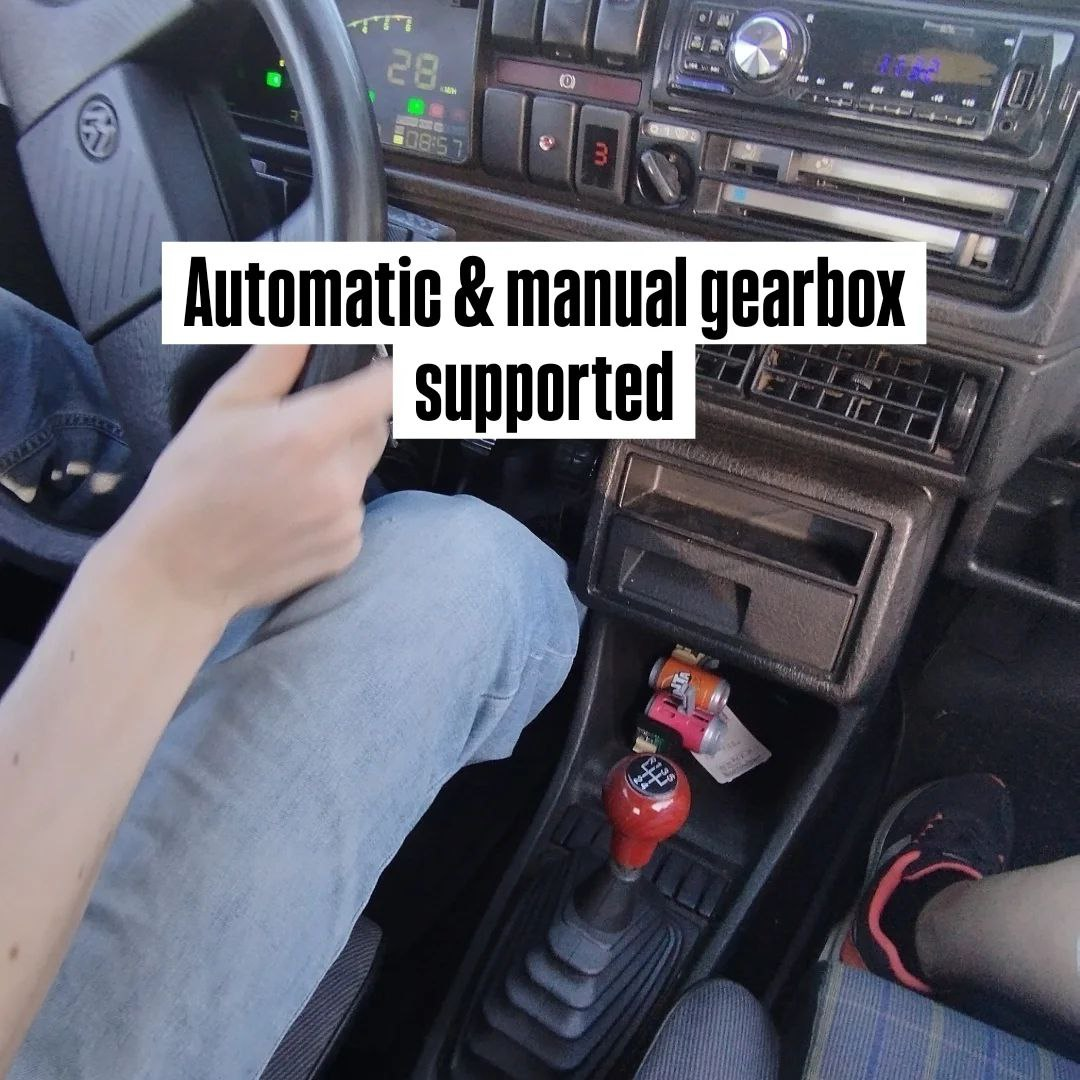
\includegraphics[width=.85\textwidth,height=.60\textheight,keepaspectratio]{figures/ivevo/image10.png}
\caption{Indicateur de rapport}
\end{figure}
\section{Lambda}
Ne pas raccorder l'indicateur à la sonde lambda d'origine du Golf 2. La source exige une sonde de mesure séparée ; si la sonde d'origine est conservée, deux sondes sont installées. Une sonde à bande étroite produit environ 0,1 V (pauvre) à 0,9 V (riche), sans mesure précise du rapport air-carburant. Le raccordement direct nécessite un étalonnage.

Une sonde large bande nécessite son propre contrôleur ; IV-Evo ne peut pas la piloter directement. La Bosch LSU 4.9 est recommandée avec un contrôleur compatible, par exemple SLC Free, DIY-EFI TinyWB, Sigma Lambda Controller Free 2 ou rusEFI wideband. Raccorder la sonde suivant les instructions du contrôleur et utiliser sa sortie analogique. Elle peut être de 0–5 V, 0,5–4,5 V ou 0–1 V ; conversion et courbe d'étalonnage doivent correspondre.

\begin{figure}[H]
\centering
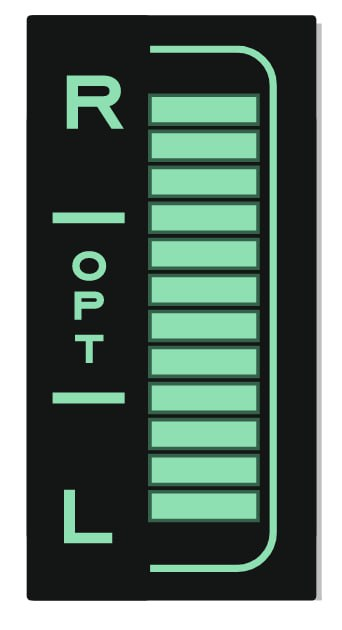
\includegraphics[width=.85\textwidth,height=.60\textheight,keepaspectratio]{figures/ivevo/image7.png}
\caption{Lambda}
\end{figure}
\section{Check Engine}
Affiche « Check Engine » lorsque la broche 2 (V2) reçoit 12 V et laisse l'écran vide à 0 V. Il s'agit d'un indicateur de signal ; aucune lecture de codes défaut ni interface OBD n'est décrite.

\begin{figure}[H]
\centering
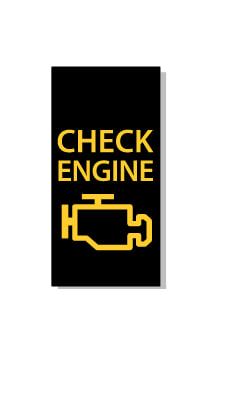
\includegraphics[width=.85\textwidth,height=.60\textheight,keepaspectratio]{figures/ivevo/image4.png}
\caption{Check Engine}
\end{figure}
\section{Pression de suralimentation (Boost)}
La source indique un capteur à trois broches, alimenté en +5 V, avec un trou de fixation et une plage de 20–250 kPa. La tension nominale de sortie est +1,8 V. La pression correspondante et la fonction de transfert complète ne sont pas fournies. Confirmer le capteur exact et sa courbe avant étalonnage ; ne pas déduire une pente d'un seul point.

\begin{figure}[H]
\centering
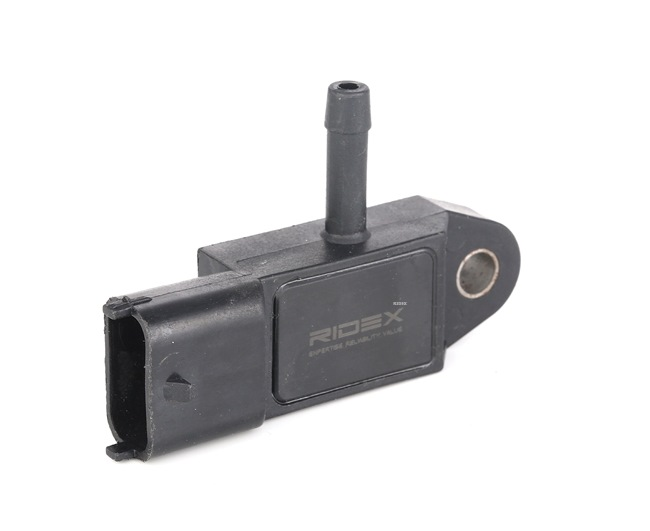
\includegraphics[width=.85\textwidth,height=.60\textheight,keepaspectratio]{figures/ivevo/image9.png}
\caption{Pression de suralimentation (Boost)}
\end{figure}
\section{Horloge}
L'application d'exemple utilise l'horloge système. L'heure n'est pas conservée au redémarrage ; sans nouveau réglage, elle sert de compteur de durée du trajet.

\begin{figure}[H]
\centering
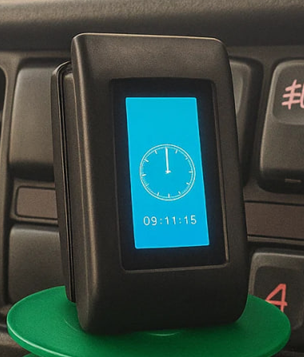
\includegraphics[width=.85\textwidth,height=.60\textheight,keepaspectratio]{figures/ivevo/image12.png}
\caption{Horloge}
\end{figure}
\section{Limites de la documentation}
Les tolérances générales d'alimentation, les températures de fonctionnement et l'indice de protection du boîtier ne sont pas fournis. Ne pas appliquer les spécifications Nano à IV-Evo.
